\section{Experimental Results and Evaluation}
\label{ch:results}

\subsection{Evaluation Methodology}
\label{sec:evalmethod}

Adjacent 60-second windows cut at a 10-second stride share 50 of their 60
rows. Split them randomly and the same seconds of driving land on both sides
of the train/test boundary; the model then recognizes drives rather than
faults, and macro-F1 inflates by 10--20 points in our measurements. Every
split in this chapter is therefore made at the level of entire recording
sessions --- a session's windows go to one side, whole --- and a regression
test in the repository fails the build if any session ever appears on both
sides. This is the one evaluation rule we treat as beyond negotiation.

We report three evaluation paths and rank them by how much trust each
deserves.

\begin{enumerate}
  \item \textbf{Fixed holdout (lowest trust).} Two sessions (drive1,
    live12) held out, the rest trained on. Fast and reproducible, but the
    39 \texttt{live} commute sessions are near-duplicates of one another
    --- the same route, driver, and car --- so a held-out \texttt{live}
    session has close siblings in training. Numbers from this path are a
    self-consistency ceiling and we do not headline them.
  \item \textbf{Leave-one-session-out (LOSO) cross-validation.} All 129
    sessions held out in turn. Honest within-vehicle, still synthetic.
  \item \textbf{Leave-one-family-out (LOFO) cross-validation.} All sessions
    of an entire family (e.g.\ every idle recording) held out together.
    This is the strongest context-transfer test the corpus supports:
    the model must classify faults in a driving context it has never seen.
  \item[--] \textbf{Real-fault evaluation (the missing path).} The only
    path that would demonstrate actual fault detection. Its evaluation code
    exists in the repository; its data folders are empty, because no public
    real-fault OBD-II recordings exist at 1\,Hz and we did not induce
    faults on our own vehicles. We list it to be explicit about what has
    \emph{not} been shown.
\end{enumerate}

One additional experiment probes the self-consistency problem directly.
The withheld-configuration test trains the classifier on faults injected
with one full parameter set (magnitudes, onset 40\,\%, ramp 15\,\%, noise
0.3) and evaluates on faults injected with a deliberately different one
(shifted magnitudes, onset 55\,\%, ramp 25\,\%, noise 0.5). Same-config
macro-F1 is 0.892; withheld-config is 0.859; the gap is 0.033. The model
is not simply memorizing one coefficient table, but the non-zero gap is a
measured reminder that some generator overfit exists.

\subsection{Classification Results}
\label{sec:classresults}

Table~\ref{tab:headline} collects the headline numbers across evaluation
paths, worst cases included.

\begin{table}[H]
  \centering
  \caption{Classifier results across evaluation paths. All numbers measure
    recovery of synthetically injected faults (self-consistency), not
    real-fault detection.}
  \label{tab:headline}
  \begin{tabular}{lcl}
    \toprule
    Evaluation & Macro-F1 & Reading\\
    \midrule
    Random Forest baseline (fixed holdout) & 1.000 & Memorization signal, not performance\\
    XGBoost (fixed holdout)                & 0.962 & Near-duplicate session leak; not headlined\\
    XGBoost LOSO mean (129 folds)          & 0.917 & Spread $\sigma = 0.084$\\
    XGBoost LOSO worst fold (live31)       & 0.699 & The honest synthetic floor\\
    XGBoost LOFO mean (5 families)         & 0.977 & Context-transfer consistency\\
    XGBoost LOFO worst family (live)       & 0.958 & \textbf{Headline number}\\
    \bottomrule
  \end{tabular}
\end{table}

Two rows in that table deserve slow reading. The Random Forest's perfect
1.000 on the earlier five-class task is the reason this book never
celebrates a high synthetic score: when your own generator writes the
answer key, perfection is a symptom. The XGBoost drop to 0.962 arrived
\emph{after} we corrected the injector's physics and added per-session
magnitude jitter --- the score went down because the task stopped being
easy to memorize, which is the direction of progress here.

We headline the LOFO worst family (0.958) and name it carefully:
\emph{context-transfer consistency}. Held out on an entire driving context
--- all 39 commute sessions, 30{,}336 windows --- the classifier still
recovers the injected faults it was trained to recognize in other contexts.
That is a real property worth having. It is not fault detection, because in
every fold, train and test faults alike were authored by the same injector.
Table~\ref{tab:lofoworst} gives the per-class breakdown for that worst
family; the full per-family table is in Appendix~\ref{app:metrics}.

\begin{table}[H]
  \centering
  \caption{Per-class F1 for the worst LOFO fold (live family held out;
    39 sessions, 30{,}336 test windows).}
  \label{tab:lofoworst}
  \begin{tabular}{lc}
    \toprule
    Class & F1\\
    \midrule
    healthy & 0.933\\
    air\_system & 0.965\\
    fuel\_system & 0.917\\
    coolant\_temp\_sensor & 1.000\\
    throttle\_position\_sensor & 0.932\\
    cold\_start & 1.000\\
    \bottomrule
  \end{tabular}
\end{table}

The LOSO distribution tells the more cautious story: a mean of 0.917 hides
a standard deviation of 0.084 and a worst fold of 0.699 (session live31).
Short sessions with unusual driving produce genuinely hard folds, and any
deployment estimate should budget for the floor, not the mean.

The per-class numbers repay a closer look, because they reveal that ``the
model'' is really six detectors of very different difficulty stapled
together. Coolant-sensor detection is effectively solved on synthetic data:
F1 sits at 1.000 in five of the six LOFO folds and never drops below 0.999.
The reason is physical and worth stating plainly --- a stuck-cold sensor
produces a coolant trajectory that simply does not occur in healthy
driving. A real engine warms monotonically toward 88--90$^{\circ}$C and
stays there; a stuck sensor holds a flat, too-low reading while everything
else about the drive looks normal. At 1\,Hz that contradiction is
unmistakable, and no amount of driving-context variation blurs it, which is
exactly why the class survives family holdout untouched.

Fuel-system detection is the mirror image, and its 0.917 F1 in the worst
family is the lowest fault-class number in Table~\ref{tab:lofofull} for a
reason. A developing fuel fault expresses through the same channel a mild
air leak does --- the fuel trims --- and in the early ramp, before LTFT has
fully integrated, the two look alike. The 0.825 precision on fuel in the
fixed-holdout breakdown (Table~\ref{tab:xgbperclass}) confirms it: the model
casts a wide net for fuel and catches some air and some healthy windows in
it. We accept this as a structural floor rather than a tuning failure. The
fuel down-weight of Section~\ref{sec:models} pulls the boundary back, but it
cannot separate two faults that genuinely share a signature during their
first thirty seconds. The honest reading is that our system distinguishes
\emph{fuel-or-air trim disturbance} from healthy very well, and resolves
\emph{which} of the two only once the fault matures.

\begin{figure}[H]
  \centering
  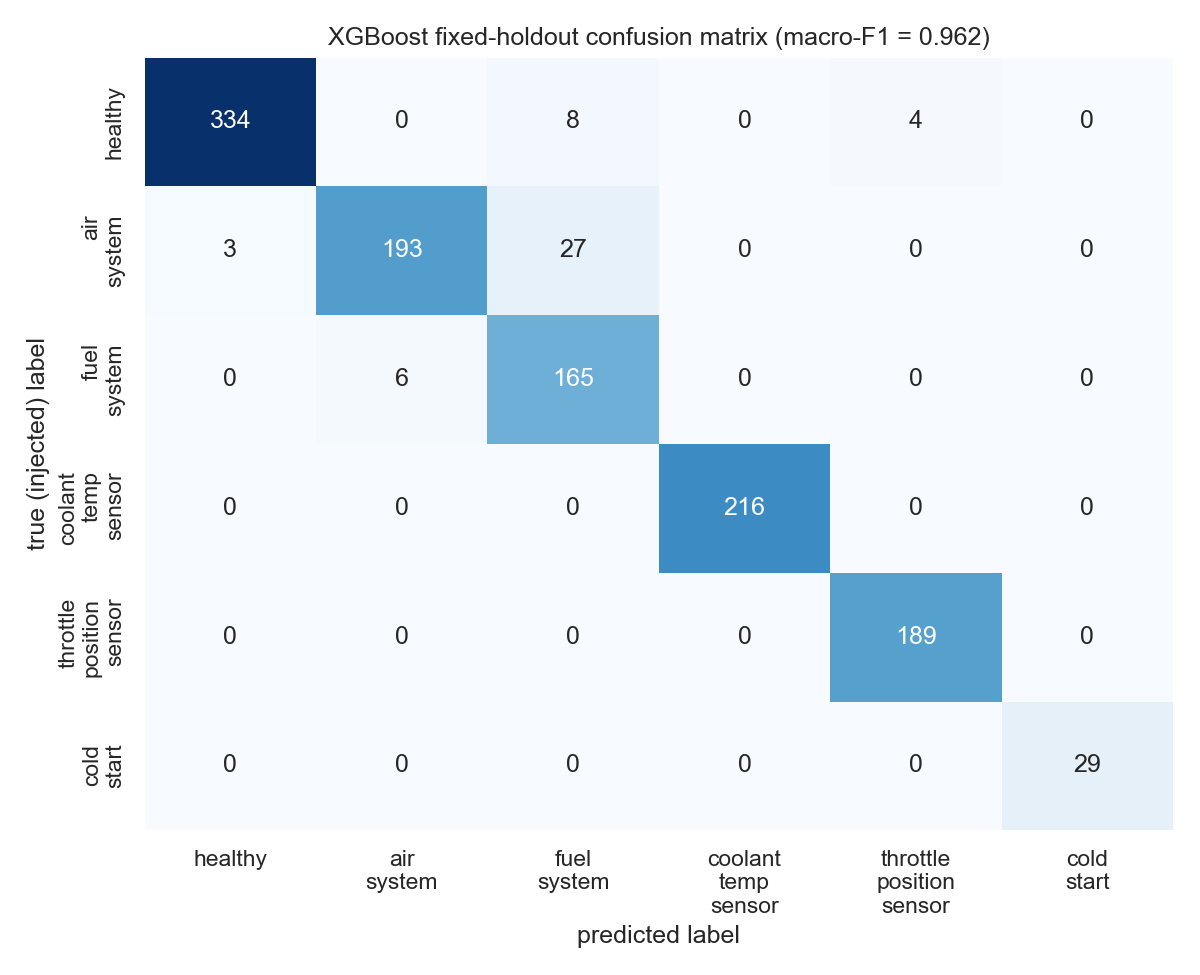
\includegraphics[width=0.85\textwidth]{fig_confusion_xgb.png}
  \caption{Fixed-holdout confusion matrix for the six-class XGBoost
    classifier (sessions drive1 + live12; macro-F1 = 0.962).}
  \label{fig:confusion}
\end{figure}

Figure~\ref{fig:confusion} shows where the errors live: almost entirely
inside a healthy--air--fuel triangle. The largest single cell is
air\_system predicted as fuel\_system (27 of 223 air windows), with smaller
flows of healthy into fuel (8) and fuel into air (6). The triangle is
physically sensible. Early-ramp air and fuel faults both surface first as
small fuel-trim disturbances at idle, and a window straddling the fault
onset is legitimately ambiguous between ``still healthy'' and ``barely
faulty.'' Coolant-sensor and cold-start windows, whose thermal signatures
are unambiguous at 1\,Hz, are never confused with anything (F1 = 1.000 and
support 216 and 29 respectively).

\subsection{Data Exploration Results}
\label{sec:eda}

The exploratory analysis below was produced by the repository's Phase-1
notebook against the recovered 129-file corpus; the figure-generation
script in \texttt{docs/book/figures/} reproduces every plot.

\begin{figure}[H]
  \centering
  \begin{subfigure}{0.48\textwidth}
    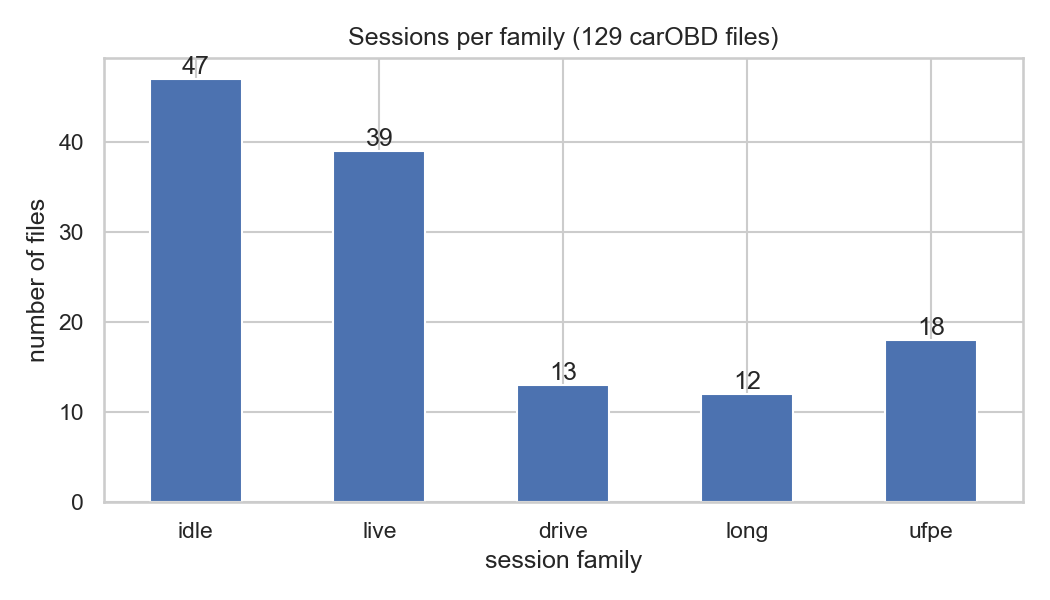
\includegraphics[width=\textwidth]{fig_family_sessions.png}
    \caption{Sessions per family.}
    \label{fig:families}
  \end{subfigure}
  \hfill
  \begin{subfigure}{0.48\textwidth}
    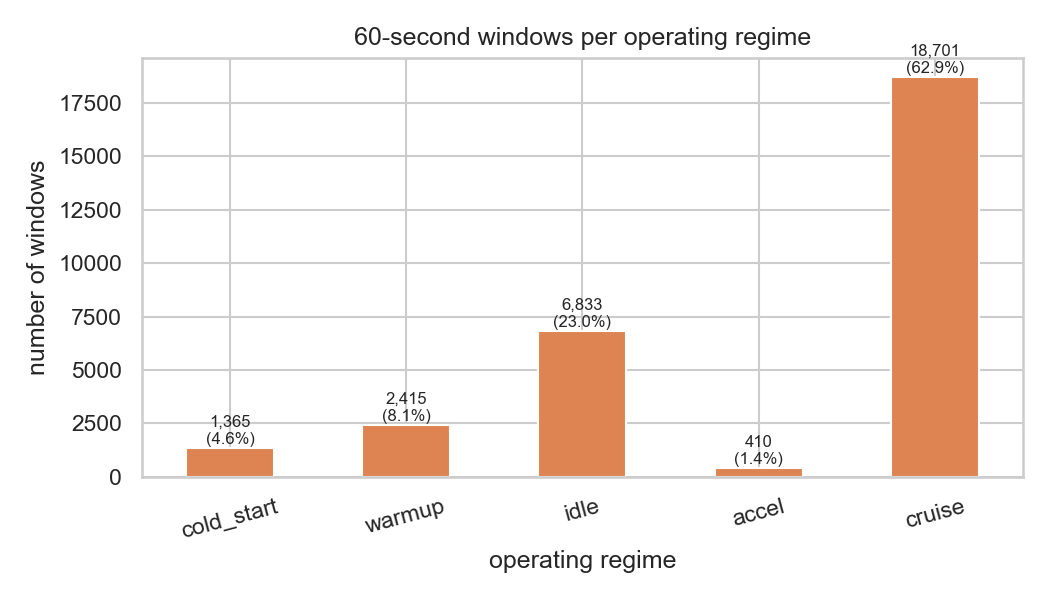
\includegraphics[width=\textwidth]{fig_regime_windows.png}
    \caption{Windows per operating regime.}
    \label{fig:regimes}
  \end{subfigure}
  \caption{Corpus composition on both axes. By file count the idle family
    dominates (47 of 129); by 60-second windows, cruise dominates (62.9\,\%)
    because driving sessions are far longer than idle ones.}
  \label{fig:composition}
\end{figure}

Composition is imbalanced on both axes, and the two axes disagree
(Figure~\ref{fig:composition}). Idle recordings are the most numerous
\emph{files}, but cruise dominates the \emph{window} count at 62.9\,\%,
followed by idle at 23.0\,\%, warm-up at 8.1\,\%, cold-start at 4.6\,\%,
and acceleration at just 1.4\,\%. The scarce regimes matter
disproportionately: a TPS fault only expresses under pedal load, and
cold-start windows are the entire training basis for that class. Class
balancing at training time addresses the label imbalance; the accel-regime
scarcity is a property of 60-second windows over real driving that
balancing cannot fix.

\begin{figure}[H]
  \centering
  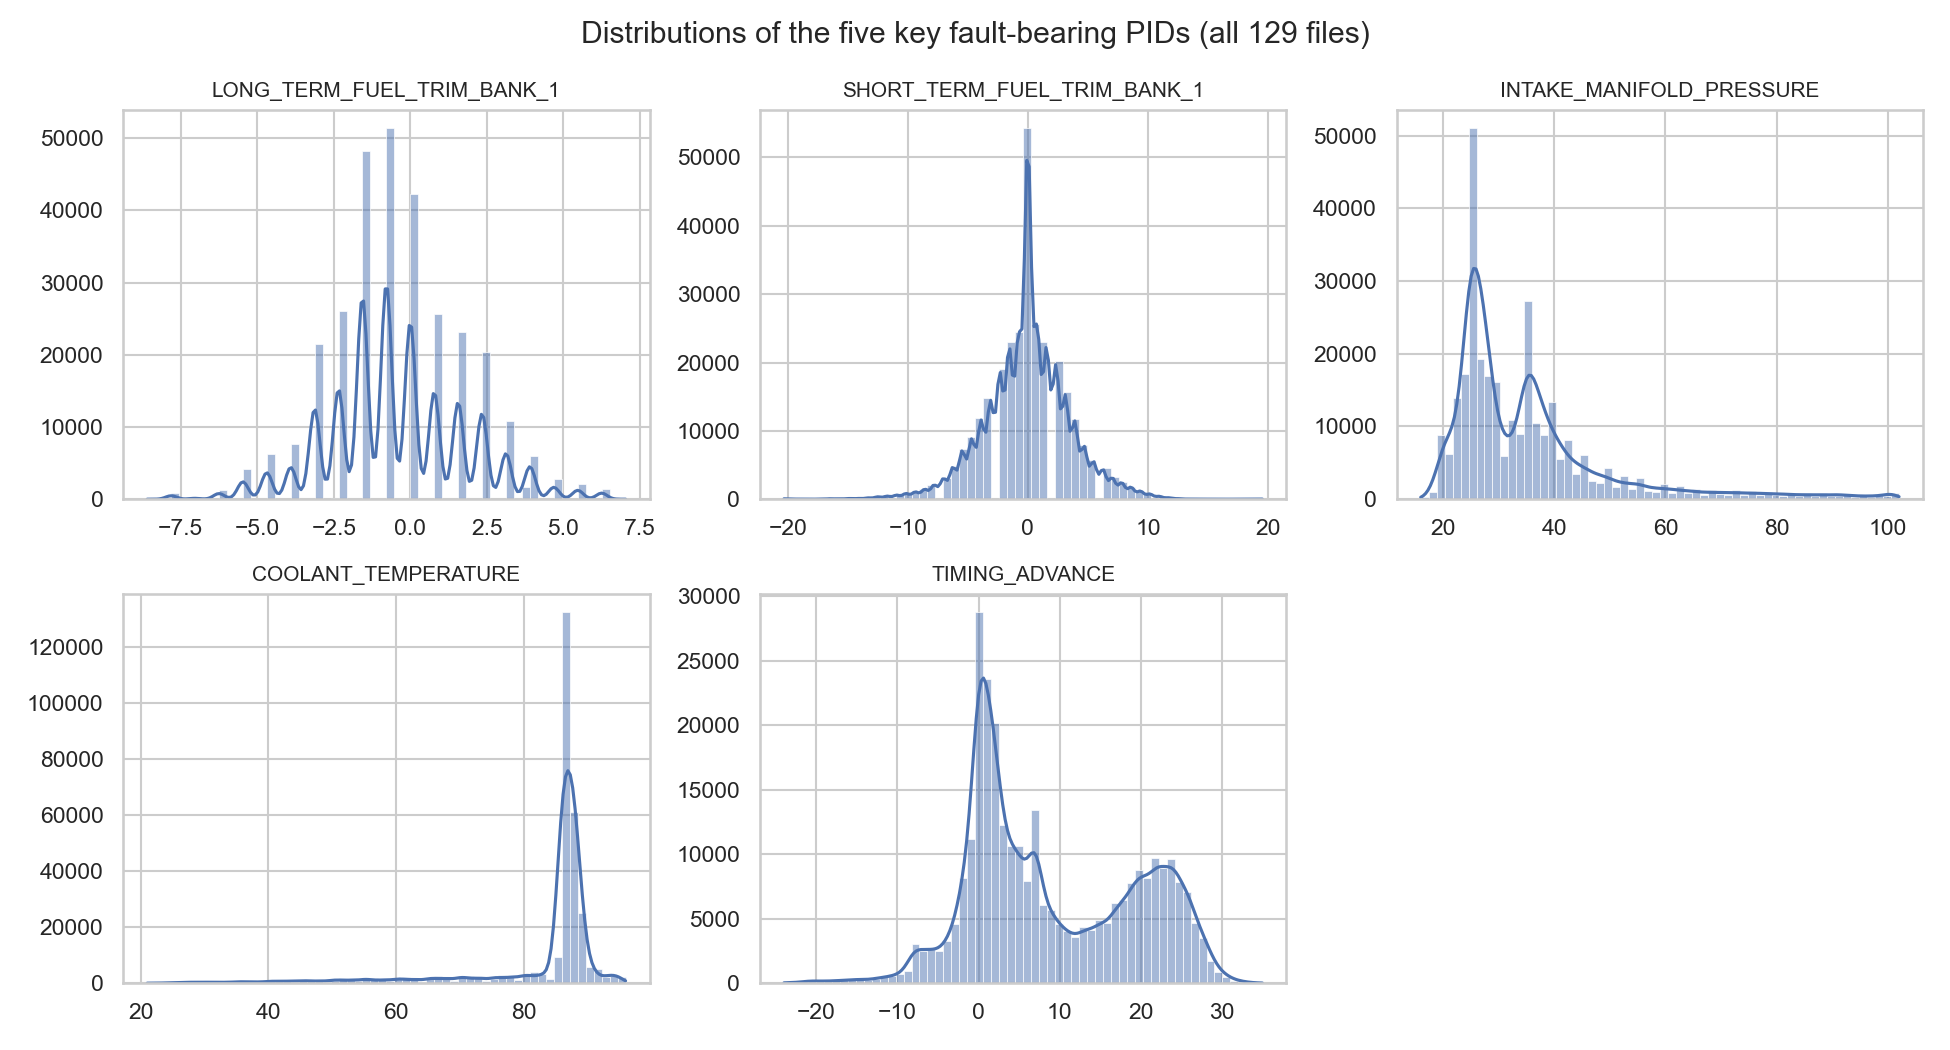
\includegraphics[width=\textwidth]{fig_fault_pid_distributions.png}
  \caption{Distributions of the five key fault-bearing PIDs across all 129
    files. Fuel trims are roughly symmetric and slightly rich-shifted with
    visible OBD-II quantization; coolant is bimodal (cold-start shoulder
    plus a warm-operation peak near 88--90$^{\circ}$C); MAP is multimodal
    from the idle/driving mixture; timing sits entirely inside its physical
    envelope.}
  \label{fig:distributions}
\end{figure}

The distribution shapes (Figure~\ref{fig:distributions}) argue for the
pipeline's normalization choice: multimodal, skewed channels do not reward
any Gaussian assumption on raw values, whereas per-vehicle z-scoring
measures displacement from the car's own mixture. The coolant bimodality
confirms cold-start data is well represented, and the timing histogram ---
bounded in $[-24^{\circ}, +35^{\circ}]$ across the entire corpus --- is
the standing proof that the column-shift repair holds
(Figure~\ref{fig:timingfix} showed the same channel reaching
776.6$^{\circ}$ under the defective parse).

\begin{figure}[H]
  \centering
  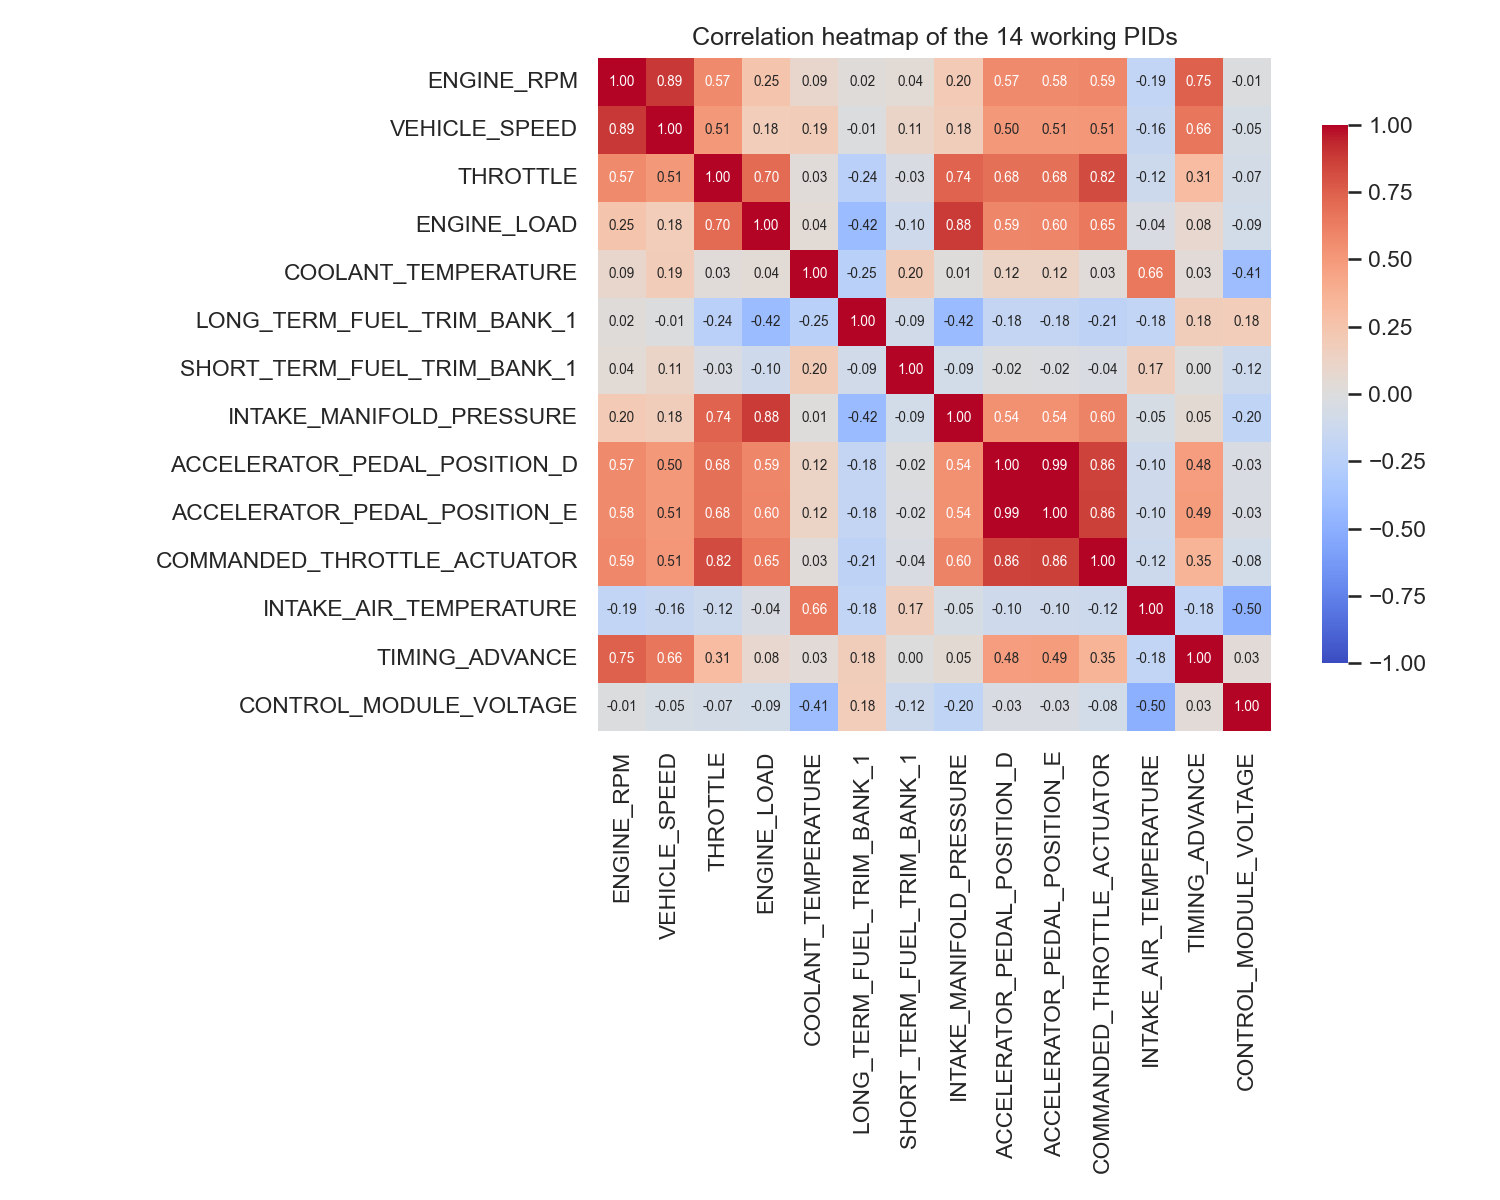
\includegraphics[width=0.9\textwidth]{fig_corr_heatmap.png}
  \caption{Correlation heatmap of the 14 working PIDs over the full corpus.}
  \label{fig:corr}
\end{figure}

The correlation structure (Figure~\ref{fig:corr}) shows the expected
physical couplings --- RPM with speed, MAP with engine load, and a tight
throttle/pedal cluster in which the two accelerator-pedal channels are
near-duplicates of each other. We keep both pedal channels despite the
redundancy: their \emph{agreement} is exactly what a TPS fault disturbs,
and the availability contract of Section~\ref{sec:dashboard} treats them as
jointly required for that class.

\begin{figure}[H]
  \centering
  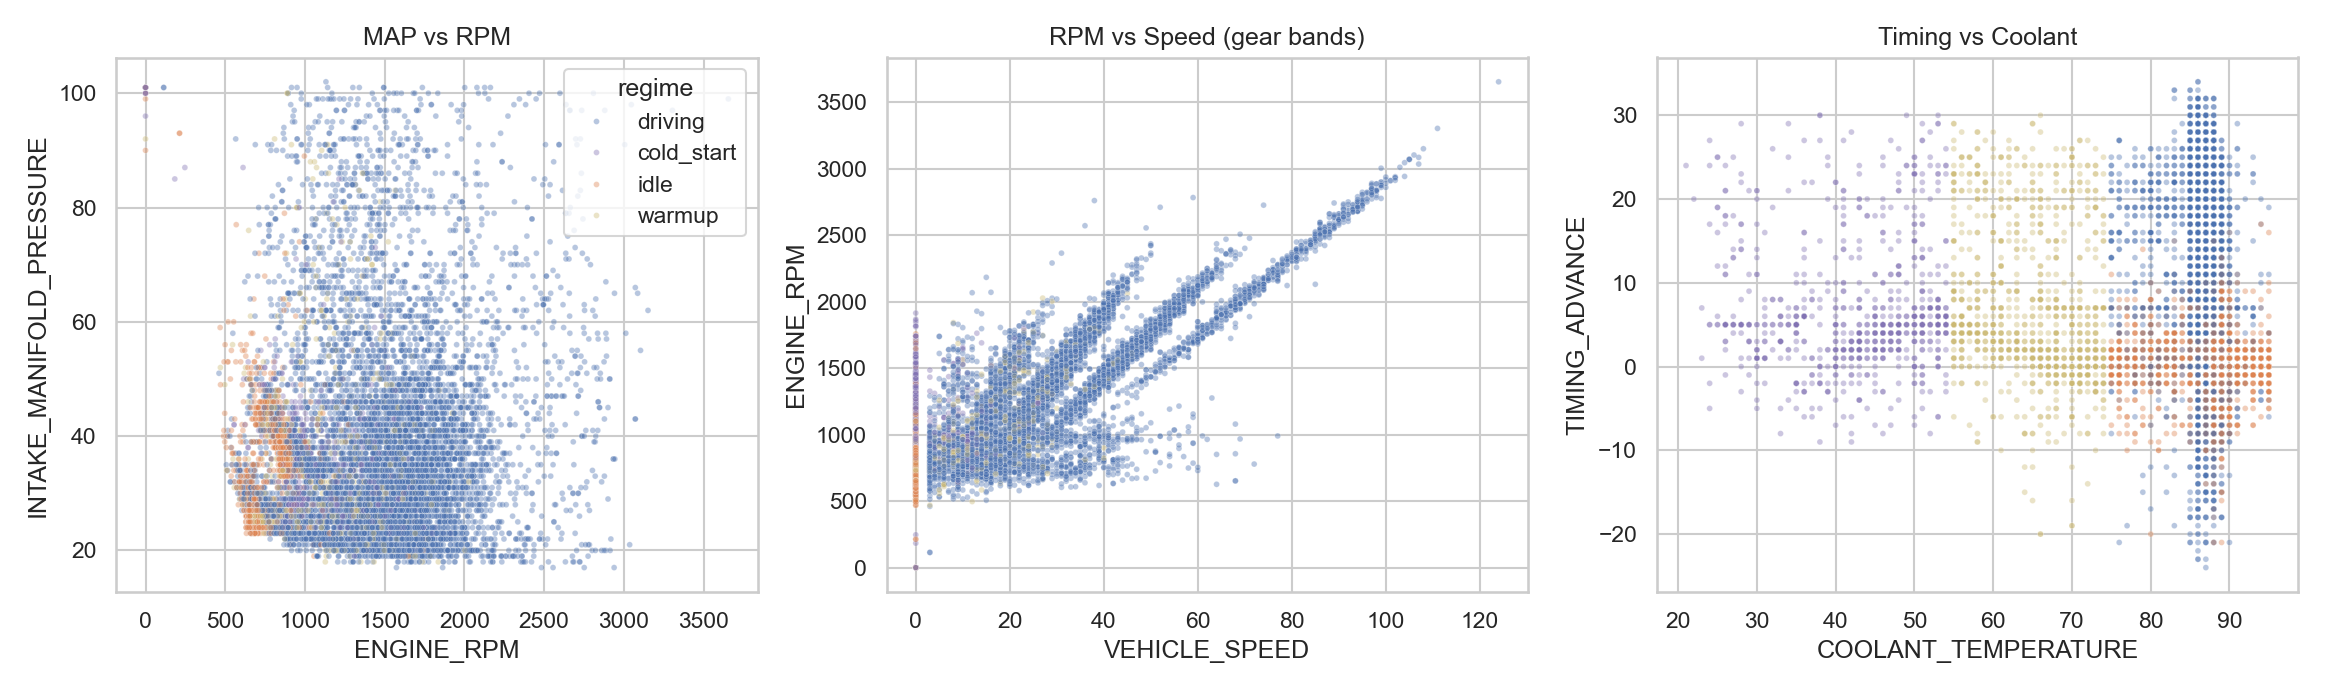
\includegraphics[width=\textwidth]{fig_bivariate.png}
  \caption{Bivariate structure, colored by a row-level regime proxy.
    Left: MAP vs RPM separates the idle cluster from the driving cloud ---
    the region the air-system fault perturbs. Center: RPM vs speed resolves
    into discrete gear bands, a drivetrain sanity check that a residual
    column shift would scramble. Right: timing advance climbs and
    stabilizes as coolant warms --- the coupling the coolant-sensor fault
    exploits.}
  \label{fig:bivariate}
\end{figure}

The bivariate views (Figure~\ref{fig:bivariate}) close the loop between
data and fault design: three of the four injected signatures are visible as
structure in the healthy data itself. Clean gear rays in the center panel
across all 129 files are also the most legible visual proof that the
recovered corpus is physically coherent. Duplicate rows, at 29{,}329
(9.6\,\%), are dominated by legitimate steady-state repeats at 1\,Hz ---
an idling engine reports the same values for many consecutive seconds ---
so we do not drop them; deleting idle repeats would distort exactly the
statistics the idle-gated air-system model depends on.

\subsection{Real-Vehicle Testing}
\label{sec:realvehicle}

The deployment target was a healthy 2015 Toyota Yaris --- a different car,
a different engine-management philosophy (MAF-based), and a different
decade from the training vehicle. Data reached the pipeline through the
OBD-LOG app and an ELM327 Bluetooth adapter. We scored two recordings:
\texttt{obd22}, a 1{,}740-row (29-minute at 1\,Hz) session used as the
baseline capture, and \texttt{transition}, a 2{,}148-row session spanning a
cold start and the transition into driving. The app's three tier captures
(124, 121, and 65 rows at parked idle) served as the throughput tests of
Table~\ref{tab:pollrate}.

The single missing channel dominates everything about this test. On both
recordings, exactly one working PID is absent: \texttt{INTAKE\_MANIFOLD\_%
PRESSURE}. The Yaris meters air with a MAF sensor and simply does not
expose PID 010B, so the MAP column is present in the CSV schema but empty
in every row.

\begin{table}[H]
  \centering
  \caption{Real-vehicle scoring outcomes on the healthy 2015 Toyota Yaris,
    with the Untested contract applied. Raw label counts are the
    classifier's per-window outputs before suppression.}
  \label{tab:yaris}
  \begin{tabular}{lcccc}
    \toprule
    Session & Rows / windows & Missing PIDs & Evaluable windows & Verdict\\
    \midrule
    obd22      & 1{,}740 / 169 & MAP only & 7 of 169 & INSUFFICIENT DATA\\
    transition & 2{,}148 / 209 & MAP only & 6 of 209 & INSUFFICIENT DATA\\
    \bottomrule
  \end{tabular}
\end{table}

Behind Table~\ref{tab:yaris} sits the incident that reshaped the system.
Before the Untested contract existed, missing MAP features were filled with
the \emph{training vehicle's} baseline values. To the classifier, a
perfectly flat, perfectly average MAP on a car whose every other channel
varied normally looked like an enormous deviation --- and the model mapped
that artifact squarely onto air\_system. The healthy Yaris scored
``97\,\% air\_system, FAULT DETECTED.'' The raw label counts still show the
shape of that failure: on \texttt{obd22}, 162 of 169 windows carry the
air\_system label (with 5 healthy, 1 fuel, 1 TPS); on \texttt{transition},
203 of 209. Fabricated sensor values produce confident wrong answers ---
that is the design lesson we consider this test's main deliverable.

With the contract in place, the same recordings produce the correct
behavior end to end: MAP-dependent features stay NaN, air\_system is
declared Untested for the session, its windows are excluded from
evaluation, and the seven (respectively six) remaining evaluable windows
fall below the ten-window floor --- so the report prints INSUFFICIENT
EVALUABLE DATA instead of a verdict. We want to be precise about what this
outcome is: it is not a failed test. The system was shown a car it cannot
fully evaluate and said so, where its predecessor invented a fault. On a
MAF-based car, honest air-system coverage requires a MAF-based feature
path, and that is future work, not a rounding error.

The channels that \emph{were} available behaved healthily. LTFT sat at
$-6.4\,\%$ mean (spread $-8.3$ to $-4.5\,\%$) across the Yaris recordings
--- a mild, steady rich bias, consistent across sessions, comfortably
inside the $\pm10\,\%$ band that our fuel-fault severity model treats as
the concern threshold, and exactly the kind of per-vehicle personality the
baseline z-scoring exists to absorb.

\subsection{Forecaster Results}
\label{sec:forecastresults}

Table~\ref{tab:forecaster} evaluates the four PID-forecaster regressors
against the persistence baseline (``the next 60 seconds change nothing''),
in z-scored units on held-out sessions.

\begin{table}[H]
  \centering
  \caption{PID forecaster mean absolute error (z-units, 60\,s horizon,
    held-out sessions) versus the persistence baseline.}
  \label{tab:forecaster}
  \begin{tabular}{lccc}
    \toprule
    Target channel & Forecaster MAE & Persistence MAE & Beats baseline?\\
    \midrule
    COOLANT\_TEMPERATURE      & 0.050 & 0.112 & Yes (2.3$\times$ better)\\
    INTAKE\_MANIFOLD\_PRESSURE & 0.773 & 0.800 & Barely\\
    THROTTLE\_TO\_PEDAL\_RATIO & 0.829 & 0.903 & Barely\\
    LONG\_TERM\_FUEL\_TRIM     & 1.152 & 0.492 & \textbf{No --- 2.3$\times$ worse}\\
    \bottomrule
  \end{tabular}
\end{table}

The pattern is physical. Coolant temperature follows slow, deterministic
thermal dynamics, and the forecaster genuinely learns them. MAP and the
throttle-to-pedal ratio are driver-driven; sixty seconds ahead, the driver
is close to unpredictable, and the forecaster only marginally beats
assuming nothing happens. LTFT is the painful row: its 60-second change on
healthy data is near-zero noise around a session-specific level, the model
overreacts to that noise, and it loses to persistence by a factor of 2.3
--- on the one channel most diagnostic of fuel faults. We keep the LTFT
regressor in the artifact set and its failure in this table, because a
reader who deploys Pillar~2 must know that the drift signal for fuel
faults comes from the anomaly detector and the classifier, not from the
forecaster. For completeness, the one-class IsolationForest scores an AUC
of 0.69 (95\,\% CI 0.66--0.72) separating healthy from any-fault windows
on the synthetic test set, and its false-positive rate on held-out healthy
sessions (15.6\,\% at the intended 1\,\% budget) is the measured argument
for per-vehicle re-fit before any live use.

\subsection{Discussion}

Three threads run through these results. First, the evaluation hierarchy
did its job: the same model that scores 1.000 (RF) or 0.962 (fixed holdout)
under leaky-adjacent conditions scores 0.699 on its worst honest fold, and
designing the report around the floor rather than the ceiling changed what
we were willing to claim. Second, the cross-vehicle test produced no
detection result at all --- and that non-result, delivered as two correct
refusals on a car the first version had confidently mislabeled, is the
strongest evidence in this book that the reporting layer works. Third,
every number above is bounded by the same asterisk: the faults were written
by our own injector. The 0.033 withheld-configuration gap says the model is
not merely memorizing coefficients; nothing in this chapter says it detects
real faults. Closing that gap needs data, not modeling, and
Section~\ref{sec:future} puts it first in line accordingly.

Read together, the classification results, the forecaster failure on LTFT,
and the Yaris deployment tell a consistent story rather than three separate
ones. Wherever a signal is slow and thermally or mechanically determined
--- coolant warm-up, timing versus temperature --- both the classifier and
the forecaster do well, because the underlying physics leaves little room
for session-specific noise to hide in. Wherever a signal reflects the
ECU's learned, car-specific fuel state --- LTFT above all --- both
components struggle, because the same absolute trim value means something
different on every car and every tank of fuel. That split is not a
coincidence of which experiments happened to work; it is the same physical
fact showing up three separate times, and it is the strongest argument in
this report for treating per-vehicle baselining as necessary rather than
optional.
